\documentclass[fleqn,12pt]{exam}
\usepackage{pifont,enumerate,url}
\usepackage{dingbat}
\usepackage{amsmath}
\usepackage{fleqn}
\usepackage{epsfig,upgreek}
\usepackage{mathptm,color}
\newcommand{\res}{\mathrm{res}}
\newenvironment{handlist}{
  \begin{enumerate}[\leftthumbsup]
    \addtolength{\itemsep}{-1.0\itemsep}}
  {\end{enumerate}}

\addpoints
\boxedpoints
\pointsinmargin
\pointname{pts}

\newcommand{\dotprod}{\, {\scriptzcriptztyle \stackrel{\bullet}{{}}}\,}
\newcommand{\complex}{\mathbf{C}}
\newcommand{\integers}{\mathbf{Z}}
\newcommand{\nat}{\mathbf{N}}
\newcommand{\imag}{\mathrm{i}}
\newcommand{\range}{\mathrm{range}}
\newcommand{\Res}{\mathrm{Res}}
\newcommand{\euler}{\mathrm{e}}
\usepackage{fourier}
%\shadedsolutions
\definecolor{SolutionColor}{rgb}{1,0.95,1}
%\definecolor{SolutionColor}{rgb}{1,1,0.7}
\addpoints
\boxedpoints
\pointsinmargin
\pointname{pts}
\newcommand{\reals}{\mathbf{R}}

\begin{document}
\large
\vspace{0.1in}
\noindent\makebox[3.0truein][l]{{\bf MATH 365}}
{\bf Name:}\hrulefill\
\noindent \makebox[3.0truein][l]{\bf Review for Exam  3}
{\bf Row and Seat:}\hrulefill\
\normalsize


\vspace{0.1in}


\begin{questions}


\question Find the radius of convergence for each series

\begin{parts}
\part [10]  $\displaystyle \sum_{k=0}^\infty \frac{1}{1+k^2} x^k$
\begin{solution}[2.0in]
\end{solution}

\part [10]  $\displaystyle \sum_{k=0}^\infty    \frac{(k!)^2}{(3 k)!} x^k$

\begin{solution}[2.0in]
\end{solution}
\end{parts}
\question [10] Use the bound
\begin{equation*}
   \left |  \int_\gamma F(z) \, \mathrm{d} z  \right| \leq \underset{z \in \gamma}{\max} |F(z)| \times \mbox{length}(\gamma)
\end{equation*}
to find an \emph{upper bound} for
\[
    \int_{L}  \frac{1}{x - \imag} \, \mathrm{d} x,
\]
where \(L\) is the line segment from \(-1  - 5 \imag\) to \(1 + 5 \imag\). 

\begin{solution}[2.5in]  A parametric representation of  \(L\) is \(z = (1 + 5 \imag) t, \, t \in [-1,1]\).  The square distance from a point on the line to \(\imag\) is
\[
   \left(  (1 + 5 \imag) t \right)  \overline{  \left(  (1 + 5 \imag) t \right)  }  =  26 t^2-10 t+1.
\]
The minimum of \(t \in [-1,1] \mapsto   26 t^2-10 t+1 \) is \(1 / 26\). Thus for \(z \in L\), we have
\[
   \frac{1}{|z - \imag|} \leq \sqrt{26}.
\]
Since the length of \(L\) is  \(2 \sqrt{26} \), we have
\[
  \left |  \int_{L}  \frac{1}{x - \imag} \, \mathrm{d} x \right | \leq \sqrt{26} \times 2 \sqrt{26} =  52.
\]
By explicit computation, we have
\[
   \left|  \int_{L}  \frac{1}{x - \imag} \, \mathrm{d} x \right | = \left | \ln(4 \imag +1) - \ln (-6 \imag-1) \right| \approx 3.08.
\]
So the upper bound is somewhat pessimistic.
\end{solution}


\question Write a critique of Billy's work
\begin{align*}
   \int_0^{2 \uppi} \frac{1}{4 + \cos(x)} \, \mathrm{d} x &= \left. \frac{2 \arctan\left( \frac{3 \sin{(x)}}{\sqrt{15}\, \left( \cos{(x)}+1\right) }\right) }{\sqrt{15}} \right|^{x = 2 \uppi}_{x=0} \\
   &= 0 - 0 \\
   &= 0.   
\end{align*}
\textbf{Fact:} Everywhere $\frac{2 \arctan\left( \frac{3 \sin{(x)}}{\sqrt{15}\, \left( \cos{(x)}+1\right) }\right) }{\sqrt{15}}$ is
differentiable, its derivative is the integrand. Here is a graph of the antiderivative.

\begin{figure*}[h]
\begin{center}
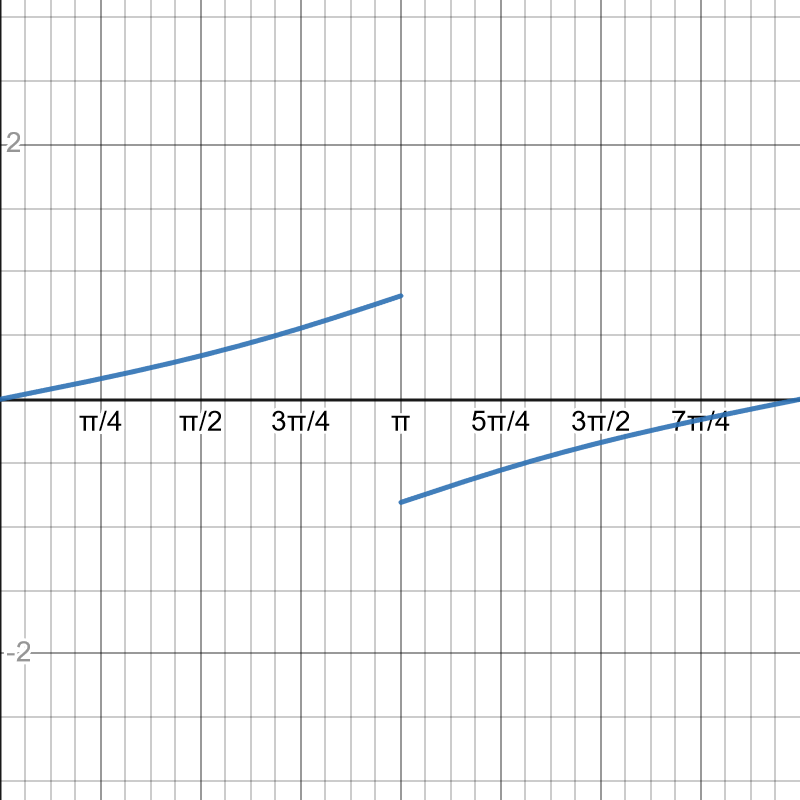
\includegraphics[scale=0.1]{desmos-graph(42)}
\caption{Graph of antiderivative on the interval $[0, 2 \uppi]$.}
\end{center}
\end{figure*}



\question Find the \emph{numerical value} of each sum.
\begin{parts}

\part[10]  \(\displaystyle \sum_{k=0}^\infty \left(\frac{2}{3} \right)^{k+1} \)
\begin{solution}[2.5in]
\[
  \sum_{k=0}^\infty \left(\frac{2}{3} \right)^{k+1} = \frac{2}{3} \sum_{k=0}^\infty \left(\frac{2}{3} \right)^{k}  = 2.
\]
\end{solution}

\part[10]  \(\displaystyle \sum_{k=2}^\infty  \left(\frac{2}{3} \right)^{k+1} \)

\begin{solution}[2.5in]
\[
  \sum_{k=2}^\infty  \left(\frac{2}{3} \right)^{k+1}  =  \sum_{k=0}^\infty  \left(\frac{2}{3} \right)^{k+3}  = \frac{8}{27}  \sum_{k=0}^\infty  \left(\frac{2}{3} \right)^{k}  = \frac{8}{27} \times  3 = \frac{8}{9}.
\]
\end{solution}

\end{parts}



\question  Find the \emph{numerical value} for each contour integral, where \(C\) is the unit circle.

\begin{parts}

\part [10] \(\displaystyle  \int_C \frac{1}{z - 5 \imag} \, \mathrm{d} z \).

 \begin{solution}[2.5in] The integrand is analyic inside the contour; so   \(\displaystyle  \int_C \frac{1}{z - 5 \imag} \, \mathrm{d} z = 0 \).
\end{solution}


\part [10] \(\displaystyle  \int_C \frac{1}{z - \imag/5} \, \mathrm{d} z \).

 \begin{solution}[2.5in] The simple pole is inside the contour; we have
 \[
     \int_C \frac{1}{z - \imag/5} \, \mathrm{d} z  = 2 \uppi \imag.
 \]
\end{solution}



\end{parts}




\question [10] For $w > 0$, find the value of 
\begin{equation}
 \int_{-\infty}^\infty \frac{1}{4 + x^2}  \euler^{\imag w x} \, \mathrm{d} x.
\end{equation}



 \begin{solution}[3.5in] For \(z > 0\),  Jordan tells us we can complete the contour  in the upper half plane:
 \[
  \frac{\euler^{\imag z x}}{4 + x^2} \, \mathrm{d} x = 2 \uppi \imag  \, \Res \left (\frac{\euler^{\imag z x}} {4 + x^2}, x = 2 \imag  \right) = \uppi \euler^{-2 z} 
 \]  
  For \(z < 0 \),  Jordan tells us we can complete the contour  in the lower half plane:
 \[
  \frac{\euler^{\imag z x}}{4 + x^2} \, \mathrm{d} x = 2 \uppi \imag  \, \Res \left (\frac{\euler^{\imag z x}} {4 + x^2}, x = -2 \imag  \right) =  \uppi \euler^{2 z} 
 \]  
\end{solution}



\question [10] My friend Pauline claims that since the function \(\mbox x \in \complex \mapsto \euler^{\euler^{\imag x}} \) is
entire, we have  
\[
  \int_0^{2 \uppi} \euler^{\euler^{\imag x}}  \, dx  = 0.
\]
Pauline  is correct that the function  \(\mbox x \mapsto \euler^{\euler^{\imag x}} \) is entire. But is Pauline  correct about the value of the integral? If not, find the correct value for this definite integral.
 \begin{solution}[3.5in]  To find the value of this integral, we convert it to a contour integral around the unit circle \(C\).  To do this, let \(z = \euler^{\imag x}\). Then \(\mathrm{d} z =
   \imag  \euler^{\imag x} \mathrm{d} x = \imag z \mathrm{d} x \).  We have
 \[
  \int_0^{2 \uppi} \euler^{\euler^{\imag x}}  \, dx = \int_C \euler^z \frac{1}{\imag z} \, \mathrm{d} z = 2 \uppi \imag \, \Res \left(\frac{\euler^z}{\imag z},z=0 \right) = 2 \uppi.
 \]
\end{solution}



\end{questions}
\end{document}

\question A function \(F\) is differentiable on \(\mathbf{C}- \{-\imag, 8 \imag\}\). At  \(-\imag \) and \(8\imag\), the
function has poles of order 42. Given that
\(
   \res(F,-\imag) = 1066 \mbox{ and }\res(F,8 \imag) = 2014
\),
find the numerical value of each of the following (remember that \(\kappa(a,r)\) is a circle centered at \(a\) with
radius \(r\) with the counterclockwise orientation).
\begin{parts}

\part [10] \(\displaystyle \int_{\kappa(0,1/2)} F(z) \, dz \)

\begin{solution}[0.5in]
\end{solution}


\part [10] \(\displaystyle \int_{\kappa(0,2014)} F(z) \, dz \)

\begin{solution}[0.5in]
\end{solution}

\end{parts}


\question [10]  Find the numerical value of \(\res \left( \frac{x^2}{\sin(x)-x}, 0 \right)\).
\begin{solution}[2.5in]
\end{solution}


\question [10] The formula for a function \(F\) is  \(\displaystyle F(z) = \sum_{k=-\infty}^\infty \frac{ z^k }{k^5 + 1}\).
Find the numerical value of \( \res(F,0) \).

\begin{solution}[2.5in]
\end{solution}



\question Find the poles of each function; at \emph{each} pole, find the residue.

\begin{parts}

\part [10] \(F(z) = \frac{\exp(29 z)}{z^2 + 1} \).

\begin{solution}[2.0in]
\end{solution}


\part [10] \(G(z) = \frac{\sqrt{z}}{(z - 1) (z-3)} \).

\begin{solution}[2.0in]
\end{solution}



\end{parts}

\newpage

\question [10] For an integer (negative, zero, or positive) \(n\), find the numerical value of \(\int_{-\pi}^{\pi} \exp(\imag n x) \, dx \).

\begin{solution}[4.0in]
\end{solution}

\newpage

\question [10] Given that \(G(x) = \sum_{k=-\infty}^{\infty} g_k \exp(\imag k x)\), where \(g_k \in \complex\) for all integers \(k\), show all
the steps, along with explanations, required to express \(g_k\) as a definite integral (integrand involves \(G\)). You calculation can
be formal, that is, make steps that are sometime true, but the conditions that justify these steps needn't be given.


\begin{solution}[5.0in]
\end{solution}

\newpage

\question [10] Find the numerical value of \(\int_{-\infty}^\infty \frac{1}{(z - 2 - 29 \imag) (z + 5 - \imag)} \, dz.\) Support the
steps of your work.
\end{questions}
\end{document}

\question [10] The Heine-Borel theorem tells us that a subset \(S\) of
the complex numbers is \emph{compact} if and only if \(S\) is
\underline{\phantom{xxxxxxxx}} and \underline{\phantom{xxxxxxxx}}.

\question Express each number \emph{explicitly} in rectangular
form. (The number \(3 + 5 i\) is in rectangular form, but the number
\(8 e^{i \tan^{-1}(1/2)} \) isn't in rectangular form.)

\begin{parts}

\part [10] \(\log(-1 + i) = \)
\begin{solution}[1.0in]

\end{solution}

\part [10] \(\log(i) = \)
\begin{solution}[1.0in]

\end{solution}

\end{parts}


\question Find the numerical value for each integral. Show all of your work (of course).
The curve \(\kappa(a,r)\) is the circle centered at \(a\) with radius \(r\), and the curve 
\([a,b]\) is
the line segment from \(a\) to \(b\). For the last question, you might like to use
\(\int \sqrt{z} \, dz = \frac{2}{3} \,{z}^{\frac{3}{2}}\) on any blob that doesn't
contain the negative real axis.

\begin{parts}

\part [10] \(\displaystyle \int_{\kappa(0,1)} \frac{1}{z} \, dz  = \)

\begin{solution}[1.0in]

\end{solution}

\part [10] \(\displaystyle \int_{\kappa(0,1)} z^{2011} \, dz  = \)
\begin{solution}[1.0in]

\end{solution}

\part [10] \(\displaystyle \int_{[-1+i,1+i]} \sqrt{z} dz  = \)
\begin{solution}[1.0in]

\end{solution}


\end{parts}



\question [10] Show that \(\log(w z) = \log(w) + \log(z)\) is not an identity.
\begin{solution}[1.0in]

\end{solution}


\question [10] Starting with
\(
  \log(x + i y) = \log \left(\sqrt{x^2 + y^2}\right) + i \tan^{-1}(y,x),
\)
find the derivative of the natural logarithm. Recall the that derivatives of the two
argument inverse tangent function are
\[
  \frac{\partial}{\partial x}  \tan^{-1}(y,x) = - \frac{y}{y^2+x^2},
   \quad \frac{\partial}{\partial y}  \tan^{-1}(y,x) =  \frac{x}{y^2+x^2}.
\] 
\begin{solution}[2.0in]

\end{solution}

\newpage
\question [10] Let \(F : \complex \to \complex\) be differentiable and let \(F = u + i v\), where
\(u\) and \(v\) are the real and imaginary parts of \(F\). Assuming that the first partial derivatives
of \(u\) and \(v\) are continuous, use the Green theorem
to show that
\(
  \int_{\partial{\left(N(0,1) \right)}} F(z) \, dz  = 0.
\)
Recall the Green theorem:
\[
  \int_{\partial(S)} u dx + v dy = \iint_S v_x - u_y \, dA.
\]

\begin{solution}[3.5in]

\end{solution}

\question [10] Let \(\mathcal{C} = \{ N(0,k) \, | k \in \mathbf{N} \}\). Thus \(\mathcal{C} = \{N(0,1), N(0,2), \dots \}\).
We have \(\underset{x \in \mathcal{C}}{\cup} x = \complex\).
Let \(\mathcal{C}^\prime\) be \emph{any} finite subset of \(\mathcal{C}\). Show that \(\mathcal{C}^\prime\) is
\emph{not} an open cover of \(\complex\).
\begin{solution}[2.5in]

\end{solution}

\newpage
\question [10] Using
\(
\mathrm{cosh}^{-1}\left( z\right) =\mathrm{log}\left( \sqrt{{z}^{2}-1}+z\right) 
\)
find a formula for the derivative of \(\mathrm{cosh}^{-1}\).

\end{questions}


\end{document}


\question [10] The range of the square root function is the right half plane along with
the positive imaginary axis. Using this fact, the solution set to \(\sqrt{z} = -1 + i\) is
\underline{\phantom{xxxxxxxxx}}.

\begin{solution} Since \( -1 + i \notin \mbox{range}(\sqrt{})\), the solution set to 
\(\sqrt{z} = -1 + i\) is \underline{\textbf{empty}}.

\end{solution}

\question Find the rectangular representation for each complex number; that is express each
complex number in the form \(a + i b\), where \(a,b \in \reals\).

\begin{parts}

\part [10] \((5 - i) (7 + i) = \)
\begin{solution}[1.2in]
\[\left( 5-i\right) \,\left( i+7\right) =36-2\,i\]
\end{solution}

\part [10] \(\frac{2 + i}{4 + i} =  \)

\begin{solution}[1.2in]
\[\frac{i+2}{i+4}=\frac{2\,i}{17}+\frac{9}{17}\]
\end{solution}
\part [10] \((2 + i) \overline{(3 - i)} = \)

\begin{solution}
\[\left( i+2\right) \,\overline{(3-i)} =5\,i+5\]
\end{solution}

\end{parts}
\question [10] Find the \emph{polar} representation for the number \(-1 + i\). Use the 
polar form to find the \emph{polar} representation for \(\sqrt{-1+i}\).
\begin{solution}[1.2in]
\[i-1=\sqrt{2}\,{e}^{\frac{3\,i\,\pi }{4}}\]
Also
\[\sqrt{-1+i} = 2^{1/4} {e}^{\frac{3\,i\,\pi }{8}}\]
\end{solution}



%\newpage

\question [10] Use the Cauchy Riemann (CR) equations to show that the function \(z \in \complex \mapsto z + \overline{z}\)
is not differentiable anywhere on \(\complex\). Remember that the CR equations are \(u_x = v_y, u_y  = -v_x\).
\begin{solution}[2.5in]
Using \(u(x,y) = 2x\) and \(v(x,y) = 0\), we have \(u_x(x,y) = 2 \neq 0 = v_y(x,y)\).
\end{solution}


\question [10] Use the limit of a Newton quotient to show that the function \(z \in \complex \mapsto z \overline{z}\)
is differentiable at zero.  To do this, you may use the fact that the conjugate is continuous everywhere; that is,
\(\displaystyle \lim_{z \to a} \overline{z} = \overline{a}\).
\begin{solution}[2.0in]
\[
 \lim_{z \to 0} \frac{z \overline{z} - 0 \overline{0}}{z - \overline{0}} = 
 \lim_{z \to 0} \frac{z \overline{z}}{z} = \lim_{z \to 0} \overline{z} = 0.
\]

\end{solution}



\question [10] Using the rule of exponents along with \(\exp(i x) = \cos(x) + i \sin(x)\) to 
show that \(\cos(2 x) = \cos^2(x) - \sin^2(x)\) is an identity.
\begin{solution}[2.5in]
\[
 \exp(2 i x) = \cos(2x) + i \sin(2x) = (\cos(x) + i \sin(x))^2 = \left(\cos^2(x) - \sin^2(x)\right) + 2 i
  \cos(x) \sin(x).
\]
So \(\cos(2 x) = \cos^2(x) - \sin^2(x)\) is an identity.
\end{solution}

\question [10] Let \(c : \naturals \to \complex\) and suppose that \(|c_k| \leq \left(\frac{1}{2}\right)^k\) for all
 \(k \in \naturals\). Show that the sequence \(U\) defined by
\(
  U_n =  \sum_{k=1}^n c_k
\)
is Cauchy. To help you start, you might like to use
\[
   |U_m - U_n| = \left |  \sum_{k = m}^{n} c_k \right| \leq  \sum_{k = m}^{n} |c_k| \leq \sum_{k = m}^{\infty} |c_k|
 \leq \sum_{k = m}^{\infty} \left(\frac{1}{2}\right)^k
\]
for integers \(m > n\).

\begin{solution} Continuing the above calculation gives
\[
 |U_m - U_n| \leq 2 \left(\frac{1}{2}\right)^m < 2 \left(\frac{1}{2}\right)^N, 
\]
where \(N > n > m\).
For every positive number \(\varepsilon\), we need \(2 \left(\frac{1}{2}\right)^N \leq \varepsilon\); thus
\(N \geq \log_2 \left(\frac{2}{\varepsilon}\right) \).  Since \(N\) is a positive integer, we may choose
\(N =  \mbox{max} \left\{0, \lceil \log_2 \left(\frac{2}{\varepsilon}\right) \rceil \right \} \).


\end{solution}


\end{questions}
\end{document}


\end{questions}
\end{document}
\question [10] Find a Laurent series centered at zero for the function \(z \in \complex - \{0\} \mapsto \frac{exp(x)}{x} \).
Express the series 

 
\end{questions}

%\question Know Theorem 5.13 and its proof (the proof is a calculation).

%\question Know the statement (but not the proof) of the Cauchy theorem; in particular, know
%the statement Theorem 6.1. Also, know the related Theorem 7.1.

\question Know how the deformation theorem works (Theorem 6.7).

\question Know what a Laurent series is and how to find them for some simple cases.

\question Know what a residue is; know how to find residues for the cases we've covered
in class.

\question Know the Liouville theorm (Theorem 7.9); given the Liouville theorem, know
the proof of the Fundamental Theorem of Algebra (page 127). Proving that \(\displaystyle \lim_{\infty} |p| =\infty\)
for any nonconstant polynomial isn't something we did in class (but we should have). If you need
this fact for the exam, you may simply use it without proof.

\question Know how to use residues to compute definite integrals of rational functions, trigonometric
functions.

\question Know what the Fourier transform is; know how to use the Jordan Lemma to compute a Fourier transform.

%\question Know how to use residues to evaluate infinite sums with rational summands. 

%\question Exercies 9.1, 9.3, 9.7, 9.14.

\question Find the poles of each function; and find the residue at each pole.

\begin{parts}

\part \(F(z) = \frac{z \exp(z)}{z^2 - 1} \).

\part \(G(z) = \frac{\sin(z)}{z \cos(z)} \).

\part \(H(z) = \frac{1}{1 - \exp(z)}\).

\end{parts}



\question  Find the Fourier transform of the function \(x \in \reals \mapsto \frac{1}{{x}^{2}+4\,x+5} \).

\question Use a change of variable along with the Cauchy integral formula to evaluate
\(\int_0^{2 \pi} \frac{x^(1/2)}{1+x^2} \, dx \).

\question My friend Larry claims that since the function \(\mbox x \mapsto \exp(\exp( i x)) \) is
entire\ that 
\[
  \int_0^{2 \pi} \exp(\exp( i x)) \, dx  = 0.
\]

Find the correct value for this definite integral; also explain to Larry the flaw in his reasoning. 

\question Find each residue

\begin{parts} 

\part [5] \(\mathrm{res} \left(\frac{z+1}{z^3 (z^2 + 1)}, z = 0 \right)  \)
\part [5] \(\mathrm{res} \left(\frac{z+1}{z^3 (z^2 + 1)}, z = -i \right) \)
\part [5] \(\mathrm{res} \left(\frac{z+1}{z^3 (z^2 + 1)}, z = i \right) \)
\part [5] \(\mathrm{res} \left(z^2 \exp(1/z), z = 0\right) \)
\end{parts}

\question [5] Find the numerical value of \(\int_0^{2 \pi} \sin(e^{i x}) \, dx \).

\question [10] Use the Cauchy integral theorem to find the numerical value of \(\displaystyle \int_0^\infty \frac{1}{1+x^4} \, dx.\)


\question [10] Use the Cauchy integral theorem and a Pac-Man  (aka a keyhole) contour to find the numerical 
value of \(\displaystyle \int_0^\infty \frac{x^{1/2}} {1+x^2} \, dx.\)

\end{questions}
\end{document}

\question Know the defintion of the logarithm function and know its properties (page 71).

\question Be able to show that \(\log^\prime (z) = \frac{1}{z}\) (page 73).

\question Know the meanings of \emph{open cover}, \emph{compact}, and \emph{finite subcover} (page 79).

\question Know that compact means closed and bounded (page 80).

\question Know how to prove that compact means bounded (Theorem 5.3, page 82).

\question Know how to find the length of a curve (Theorem 5.9, page 86). 

\question Know the fact expressed by Equation 5.8, page 91.

\question Understand that integrals are independent of parameterization (classnotes only, I think).

\question Know Theorem 5.19; be able to apply this theorem (Example 5.21, for example).

\question Know Theorem 5.23 and its proof.

\question Know Theorem 5.25 and its proof.

\question Know the definition of uniform convergence.

\question Know what the Green theorem is and how to use it to prove (a weak form) of 
the Cauchy theorem.

\question Know Theorem 6.2.

\question  Fill in the blanks with distinct words that have a mathematical meaning:\footnote{A 
smart-aleck answer such as ``compact'' or ``difficult to understand'' will earn you zero points.}
A compact subset of the complex numbers is \underline{\phantom{xxxxxxxxx}} and
\underline{\phantom{xxxxxxxxx}}. 

\question Express each number in rectangular form

\begin{parts}

\part  \(\log(-1) = \)

%\begin{solution}[1.0in]
%\end{solution}

\part  \(\log \left(1 + i \right) = \)
\begin{solution}[1.0in]
\end{solution}


\part  \(\sqrt{1 + i} = \)
%\begin{solution}[1.0in]
%\end{solution}
\end{parts}

\question  The inverse hyperbolic sine function has a representation in terms of 
the logarithim:
\[
   \mathrm{sinh}^{-1} = z \in \complex \mapsto \mathrm{log}\left( \sqrt{{z}^{2}+1}+z\right).
\]
Use this formula to find a formula for the \emph{derivative} of \(\sinh^{-1}\).

%\begin{solution}[2.0in]
%\end{solution}



\question  Using the fact that \(\sqrt{}\) is not differentiable
on the negative real axis, explain why inverse hyperbolic sine
function is not differentiable at \(2 i\).

%\begin{solution}[2.0in]
%\end{solution}


\question  Show that \(\log(z w) = \log(z) + \log(w)\) isn't an identity.

\begin{solution} We have
\(
  \log((-1) (-1)) = \log (1) = 0,
\)
but
\(
  \log(1) + \log(-1) = 0 + i \pi.
\)
\end{solution}

\question  Let \(\gamma = t \in [-1,1] \mapsto 1 + i t\). Find the
numerical value of \(\int_{\gamma^\star} \frac{1}{z} \, dz \).

\begin{solution}
\end{solution}

\question  Let \(\gamma = t \in [0, 2 \pi] \mapsto \exp(i t) \). Find
the numerical value of \(\int_{\gamma^\star} \sqrt{z} \, dz \).
\begin{solution}
\end{solution}


\begin{solution}
\end{solution}


\question  Let \(\gamma^\star\) be the line segment from \(\pi - i\) to \(\pi + i\). Find
the numerical value of \(\int_{\gamma^\star} \sin(z) \, dz \).

\begin{solution}
\end{solution}



\question Know how to express the integral of a complex valued function over a curve as
a Riemann integral (Eq 5.6, page 89).

\question For curves know the means of \emph{closed curve} amd \emph{simple curve} (page 84).


\end{questions}
\end{document}

